\documentclass{article}

% ====== PACKAGES D'ORIGINE ======
\usepackage{graphicx} % Required for inserting images
\usepackage{eso-pic}
\usepackage{fancyhdr}
\usepackage{geometry}
\geometry{hmargin=2.5cm}
\usepackage[squaren,Gray]{SIunits}
\usepackage{amsmath}
\usepackage[french]{babel}
\usepackage[utf8]{inputenc}
\usepackage[T1]{fontenc}
\usepackage[export]{adjustbox}
\usepackage{subcaption}
\usepackage{amssymb}
\usepackage{tcolorbox}
\usepackage{listings}
\usepackage{fontawesome5}
\usepackage{hyperref}
\usepackage{color}

% ====== AJOUTS SÛRS (pas de conflit) ======
\usepackage{csquotes} % guillemets corrects (requis par biblatex)
\usepackage{booktabs} % beaux tableaux
\usepackage[backend=biber,style=authoryear,maxnames=6,doi=false,isbn=false,url=true]{biblatex}

% ====== BIBLIO (dans le préambule pour \printbibliography) ======
\begin{filecontents}{\jobname.bib}
@inproceedings{Shazeer2017,
  title       = {Outrageously Large Neural Networks: The Sparsely-Gated Mixture-of-Experts Layer},
  author      = {Noam Shazeer and others},
  year        = {2017},
  booktitle   = {ICLR},
  url         = {https://arxiv.org/abs/1701.06538}
}
@article{Lepikhin2020,
  title       = {GShard: Scaling Giant Models with Conditional Computation and Automatic Sharding},
  author      = {Dmitry Lepikhin and others},
  year        = {2020},
  journal     = {arXiv preprint},
  eprint      = {2006.16668},
  url         = {https://arxiv.org/abs/2006.16668}
}
@article{Fedus2021,
  title       = {Switch Transformers: Scaling to Trillion Parameter Models with Simple and Efficient Sparsity},
  author      = {William Fedus and Barret Zoph and Noam Shazeer},
  year        = {2021},
  journal     = {arXiv preprint},
  eprint      = {2101.03961},
  url         = {https://arxiv.org/abs/2101.03961}
}
@article{Du2022glam,
  title       = {GLaM: Efficient Scaling of Language Models with Mixture-of-Experts},
  author      = {Nan Du and others},
  year        = {2022},
  journal     = {arXiv preprint},
  eprint      = {2112.06905},
  url         = {https://arxiv.org/abs/2112.06905}
}
@article{Cai2024,
  title       = {A Survey on Mixture of Experts in Large Language Models},
  author      = {Wenqi Cai and others},
  year        = {2024},
  journal     = {arXiv preprint},
  eprint      = {2407.06204},
  url         = {https://arxiv.org/abs/2407.06204}
}
@article{Shlens2014,
  title       = {A Tutorial on Principal Component Analysis},
  author      = {Jonathon Shlens},
  year        = {2014},
  journal     = {arXiv preprint},
  eprint      = {1404.1100},
  url         = {https://arxiv.org/abs/1404.1100}
}
@article{Greff2015,
  title       = {LSTM: A Search Space Odyssey},
  author      = {Klaus Greff and others},
  year        = {2015},
  journal     = {arXiv preprint},
  eprint      = {1503.04069},
  url         = {https://arxiv.org/abs/1503.04069}
}
@article{Kingma2014,
  title       = {Adam: A Method for Stochastic Optimization},
  author      = {Diederik P. Kingma and Jimmy Ba},
  year        = {2014},
  journal     = {arXiv preprint},
  eprint      = {1412.6980},
  url         = {https://arxiv.org/abs/1412.6980}
}
@inproceedings{Rajbhandari2023DeepSpeedMoE,
  title       = {DeepSpeed MoE: Advancing Mixture-of-Experts Inference and Training to Power Next-Generation AI Scale},
  author      = {Samyam Rajbhandari and others},
  year        = {2023},
  booktitle   = {ICML},
  url         = {https://arxiv.org/abs/2207.00032}
}
@article{Kim2023expertflow,
  title       = {expertflow: Transparent and Efficient MoE Inference via Expert Flow Prediction},
  author      = {Taewook Kim and others},
  year        = {2023},
  journal     = {arXiv preprint},
  eprint      = {2310.08402},
  url         = {https://arxiv.org/abs/2310.08402}
}
\end{filecontents}
\addbibresource{\jobname.bib}

% ====== LISTINGS (inchangé) ======
\definecolor{mygreen}{rgb}{0,0.6,0}
\definecolor{mygray}{rgb}{0.5,0.5,0.5}
\definecolor{mymauve}{rgb}{0.58,0,0.82}
\lstset{
    backgroundcolor=\color{white},   
    basicstyle=\footnotesize\ttfamily,
    breakatwhitespace=false,
    breaklines=true,
    captionpos=b,
    commentstyle=\color{mygreen},
    keywordstyle=\color{blue},
    stringstyle=\color{mymauve},
    numbers=left,
    numberstyle=\tiny\color{mygray},
    stepnumber=1,
    numbersep=5pt,
    tabsize=4,
    showspaces=false,
    showstringspaces=false,
    showtabs=false,
    frame=single,
    language=Matlab
}

% ====== MACROS ======
\newcommand{\HRule}{\rule{\linewidth}{0.5mm}}
\newcommand{\blap}[1]{\vbox to 0pt{#1\vss}}
\newcommand\AtUpperLeftCorner[3]{%
  \put(\LenToUnit{#1},\LenToUnit{\dimexpr\paperheight-#2}){\blap{#3}}%
}
\newcommand\AtUpperRightCorner[3]{%
  \put(\LenToUnit{\dimexpr\paperwidth-#1},\LenToUnit{\dimexpr\paperheight-#2}){\blap{\llap{#3}}}%
}

% Figures protégées (pas d'erreur si fichier manquant)
\newcommand{\maybegraphics}[2][]{%
  \IfFileExists{#2}{\includegraphics[#1]{#2}}{%
    \begin{tcolorbox}[colback=yellow!5,colframe=yellow!50!black]
      Image manquante: \texttt{#2}
    \end{tcolorbox}}}

\title{\Huge{Mixture of expert in LLMs}}
\author{Pierre-Louis Filoche}
\date{Mai - Juillet 2025}
\makeatletter
\pagestyle{fancy}
\geometry{hmargin=2.5cm, vmargin=2cm, footskip=0.5cm}

\begin{document}

% ====== PAGE DE GARDE ======
\begin{titlepage}
    \enlargethispage{2cm}  
    \AddToShipoutPicture{
        \AtUpperLeftCorner{1.5cm}{2cm}{\maybegraphics[width = 9cm]{logo/logo_ens.png}}
        \AtUpperRightCorner{1.25cm}{1.5cm}{\maybegraphics[width = 7cm]{logo/logo_ills.png}}
        \AtUpperLeftCorner{8cm}{23cm}{\maybegraphics[width = 3cm]{logo/logo_mila.png}}
        \AtUpperRightCorner{8cm}{23cm}{\maybegraphics[width = 1.5cm]{logo/ets.png}}
    } 
    \begin{center}
        \vspace*{8cm}
        \textsc{\@title}
        \HRule
        \vspace{1cm}
        \Huge{Rapport de stage}
        \Large{\@date}
        \vspace{1cm}
        \LARGE{\@author}
        \Large{Supervisé par Loris Marchal et Pablo Piantanida}
    \end{center}
\end{titlepage}
\ClearShipoutPicture

\fancyhead[L]{%
  \maybegraphics[width=2cm,height=\paperheight,keepaspectratio]{logo/logo_ens.png}%
  \maybegraphics[width=1.6cm,height=\paperheight,keepaspectratio]{logo/logo_ills.png}}
\fancyfoot[R]{Rapport de Stage}
\fancyfoot[L]{\@author}

\tableofcontents
\newpage



% =============================================================
\section{Introduction}

\noindent
Depuis plus de trente ans, \emph{scaler} la taille des réseaux de neurones a été l’une des stratégies les plus sûres pour améliorer leurs performances : plus de données, plus de paramètres, de meilleurs résultats. Cependant à chaque augmentation de taille des réseaux, la taille des calculs et de la mémoire nécessaire. Dans le contexte des grands modèles de langage (LLM), cette tension devient critique : on souhaite des milliards, voire des centaines de milliards de paramètres, sans pour autant multiplier d’autant le coût d’inférence.  C’est précisément pour résoudre ce dilemme qu’a été introduite l’architecture \emph{Mixture of Experts} (MoE) \cite{shazeer2017outrageously}.  

\vspace{0.4em}
\noindent
Le principe est conceptuellement simple : \textbf{ne pas activer tous les paramètres du réseau pour chaque token}.  Le cœur d’un bloc MoE est un ensemble d’\texttt{experts}, des sous‐réseaux feed-forward indépendants, et un réseau de routage.
la \texttt{gating-function} (réseau de routage) choisit un sous‐ensemble réduit d’experts à exécuter pour chaque couche.  Cette activation \emph{sparse} permet d’augmenter la capacité totale (nombre de paramètres) sans augmenter proportionnellement les flottantes‐opérations, réalisant ainsi le slogan « \emph{capacity without compute} ».  Historiquement, les premières versions d’experts remontent aux années 1990 \cite{jacobs1991adaptive}, mais c’est l’explosion des besoins de capacité dans les LLM qui a ravivé l’intérêt pour les MoE \cite{fedus2021switch}.  

\vspace{0.4em}
\noindent
Outre leur efficacité, les MoE présentent deux atouts essentiels :

\begin{enumerate}
  \item \textbf{Spécialisation émergente.} Sous la pression de l’apprentissage, les experts apprennent souvent des compétences différentes (syntaxe, ponctuation, entités rares, etc.), comme l’ont montré des analyses récentes \cite{lo2024closer, antoine2025pos}. Comprendre et contrôler ce phénomène est aujourd’hui un sujet de recherche actif.
  \item \textbf{Flexibilité systèmes.} Comme seuls quelques experts sont chargés en mémoire GPU à chaque pas, on peut déporter les autres sur CPU / SSD \cite{he2024expertflow, zhong2024adapmoe} ou adopter des stratégies de quantification agressives \cite{tang2024hobbit}, ouvrant la voie à des déploiements sur matériel contraint.
\end{enumerate}

\vspace{0.4em}
\noindent
Cependant, cette parcimonie pose aussi de nouveaux défis : équilibrage de charge entre experts, stabilité de l’entraînement, sécurité (fuites d’information par le routage \cite{yona2024stealing}) ou encore intégrité face aux attaques par débordement de capacité.  Les chapitres qui suivent analyseront ces questions et détailleront notre propre exploration des MoE, menée sur l’infrastructure Grid’5000 avec le modèle \texttt{Mixtral-8$\times$7B}.

\vspace{0.4em}
\noindent
Ainsi, les MoE s’imposent aujourd’hui comme une réponse pragmatique à la course à l’échelle : ils réconcilient l’appétit paramétrique des LLM avec les contraintes très réelles de calcul et de mémoire, tout en ouvrant un champ fertile pour la recherche sur la modularité et l’explicabilité des réseaux de neurones.

\bibliographystyle{unsrt}
\bibliography{biblio}


\subsection{Motivations}
Les architectures \emph{Mixture-of-Experts} (MoE) améliorent la capacité des LLM à coût d'inférence quasi-constant en activant seulement quelques experts par token et par couche via un routage top-$k$ \parencite{Shazeer2017, Lepikhin2020, Fedus2021, Du2022glam, Cai2024}. 
Ce stage adresse deux enjeux : (i) \textbf{opérationnel} — prédire \emph{à l'avance} quels experts seront sollicités pour \emph{précharger} et lisser la latence ; (ii) \textbf{scientifique} — quantifier la part d'information contenue dans le contexte court sur le choix des experts (stabilité, spécialisation).

\subsection{Contributions et plan}
Nous (1) mettons en place un pipeline d'extraction des trajectoires d'experts (Mixtral 8×7B), (2) évaluons des \textbf{prédicteurs déterministes} (statistiques de fréquences), (3) entraînons un \textbf{MLP léger} (V1) puis un \textbf{LSTM} (V2) opérant sur des \textbf{embeddings réduits} (PCA ou couche linéaire apprise), et (4) analysons les compromis précision/latence.

% =============================================================
\section{Environnement de travail}

\subsection{Infrastructure Grid'5000}
Les expériences ont été conduites sur la grille Grid'5000, principalement sur les sites de Rennes et Lille, avec un quota de \SI{300}{\giga\byte} de stockage dédié. Les jobs — souvent multi-heures sur GPU A100 80~Go — ont été soumis via \texttt{oarsub}, catégorie \texttt{p1}.

\subsection{Modèle étudié : Mixtral 8×7B}
\begin{itemize}
  \item \textbf{Taille totale} : 47 milliards de paramètres (dont 13~B actifs par passage).
  \item \textbf{Architecture} : 32~couches, 8~experts par couche, top-2 routing.
  \item \textbf{Implémentation} : \texttt{huggingface/transformers} (commit \texttt{v4.41.0}).
  \item \textbf{Mémoire} : \SI{45}{\giga\byte} en demi-précision.
\end{itemize}

% =============================================================
\section{État de l'art}\label{sec:etat_art}

\subsection{Gating et routage}
Le routage top-$k$ attribue à chaque jeton un score par expert, puis ne conserve que les $k$ meilleurs \parencite{Shazeer2017, Lepikhin2020, Fedus2021, Du2022glam}. Des pertes auxiliaires d'équilibrage limitent la \emph{collapse} d'experts. Le panorama récent est présenté par \textcite{Cai2024}.

\subsection{Prédiction des experts et caching}
Peu de travaux ciblent la prédiction prospective des experts ; on trouve toutefois des idées connexes de \emph{router caching} ou d’\emph{expert flow prediction} \parencite{Rajbhandari2023DeepSpeedMoE, Kim2023expertflow}.

% =============================================================
\section{Problématique et objectifs}

\textbf{Problème.} Étant donné un contexte court $(t\!-\!n,\dots,t\!-\!1)$, prédire pour le token $t$ et pour chaque couche $1..32$ la \textbf{paire top-2 d’experts} activée par le routeur.

\noindent
\textbf{Objectifs.}
\begin{itemize}
  \item Quantifier le \emph{signal} utile du contexte (tokens bruts vs embeddings).
  \item Comparer les réductions d'embeddings : \textbf{PCA} \parencite{Shlens2014} vs \textbf{couche linéaire apprise}.
  \item Évaluer l’apport d’un \textbf{LSTM} \parencite{Greff2015} face au MLP (V1).
\end{itemize}

% =============================================================
\section{Données et pipeline d'extraction}

\subsection{Sorties collectées}
Pour chaque token : \texttt{token\_id}, \texttt{router\_logits} $(32\times 8)$, \texttt{hidden\_states} $(32\times 4096)$, \texttt{embedding} $(4096)$. Les paires top-2 sont déduites des logits couche par couche.

\subsection{Jeux de données}
\texttt{helpful\_instructions} (10k prompts, $\sim$630k tokens). Distribution de fréquences très décroissante (longue traîne), qui influe sur les statistiques d’$n$-grammes.

\subsection{Prétraitements}
\begin{itemize}
  \item Trajectoires par token (séquence de paires d’experts).
  \item Matrices de co-occurrence inter-couches (28 paires possibles en top-2 pour $E=8$), normalisation par ligne (conditionnelle) et globale (conjointe).
  \item Heatmaps d’utilisation par couche (globales, par token spécifique, conditionnées par token précédent).
\end{itemize}

% =============================================================
\section{Méthodologie}

\subsection{Extraction des trajectoires}
Un script \texttt{Generate\_output.py} produit, pour chaque token d'un jeu de données, un tuple :
\begin{center}
\verb|[token_id, router_logits_{32×8}, hidden_states_{33×4096}]|.
\end{center}
Ces tenseurs sont stockés au format \texttt{.pt} et post-traités par \texttt{Stat\_experts.py} afin de récupérer, pour chaque couche~$\ell$, la paire $(e^{(1)}_{\ell}, e^{(2)}_{\ell})$ effectivement sélectionnée.

\subsection{Approche 1 : gating inter-couches}
À la couche $k$, on ré-injecte le \emph{hidden vector} $h_{k}$ dans la fonction de gating de la couche $k\!+\!n$ pour estimer la distribution $\hat p_{e}$ des experts futurs (figure~\ref{fig:gating}). La prédiction \textbf{top-1} est jugée correcte si l'expert le plus probable appartient à la paire réelle.

\begin{figure}[ht]
  \centering
  \IfFileExists{figures/schema_gating.pdf}{%
    \includegraphics[width=.8\linewidth]{figures/schema_gating.pdf}%
  }{%
    \begin{tcolorbox}[colback=yellow!5,colframe=yellow!50!black]
      Figure manquante: \texttt{figures/schema_gating.pdf}
    \end{tcolorbox}}
  \caption{Principe de la prédiction spatiale à une couche d'avance.}
  \label{fig:gating}
\end{figure}

\subsection{Approche 2 : réseau prédictif léger (V1 MLP)}
\textit{Motivation.} Généraliser au-delà des tables de fréquences (bigrammes/trigrammes rares) avec un modèle compact.  
\textit{Architecture.} Deux couches linéaires + ReLU ; sortie $32\times 8$ (ou $32\times 28$).  
\textit{Limites.} Données déséquilibrées ; risque de \emph{cheating} si les experts du contexte figurent parmi les entrées (d’où leur retrait en V2).

\subsection{Approche 3 : statistiques de co-occurrence}
La matrice $\mathbf{C}_{ij}=\mathbb P\big((e^{(1)},e^{(2)})_{\ell}=i,\,(e^{(1)},e^{(2)})_{\ell+1}=j\big)$ est estimée par comptage sur $\sim$630\,000 tokens. Deux normalisations comparées : (i) par lignes (conditionnelle) et (ii) globale (conjointe).

% =============================================================
\section{Développement : V1 $\rightarrow$ V2}

\subsection{Prédicteurs déterministes (fréquences)}
Profondeur $1$ (par token) puis $2/3/5$ (par $n$-gramme). \textit{Motivation} : baseline interprétable. \textit{Résultat} : bon signal sur tokens fréquents ; chute lorsque $t$ est retiré de l’entrée (prédire $t$ à partir de $t-n..t-1$ seulement).

\subsection{V1 — MLP léger}
\textit{But} : capacité de généralisation modérée à coût réduit. \textit{Résultat (indicatif)} : \emph{hit rate} top-2 $\approx 0.51$ — au-dessus de l’aléatoire ($\approx 0.25$) mais inférieur aux heuristiques déterministes sur tokens fréquents.

\subsection{V2 — LSTM + réduction d’embeddings}
\paragraph{Motivation} Capturer l’ordre/dynamique du contexte via un \textbf{LSTM}, tout en exploitant l’information sémantique des \textbf{embeddings} (4096 dim) après réduction.
\paragraph{PCA (offline)} Projection $4096\to d$ apprise sur \textbf{les $\sim$630k occurrences} du dataset (pondération implicite des tokens fréquents). Avantage : coût d’inférence minimal ; limite : non spécifique à la tâche (maximise variance) \parencite{Shlens2014}.
\paragraph{Couche linéaire apprise} Réduction $4096\to d$ en tête de réseau, entraînée \emph{end-to-end}. Avantage : spécifique à la tâche ; coût d’inférence légèrement supérieur (souvent marginal).
\paragraph{Implémentation} Entrée : embeddings réduits du contexte $(t\!-\!n,\dots,t\!-\!1)$ ; LSTM 1–2 couches ($h\in\{128,256,512\}$) ; sortie par couche : $28$ classes (paire) ou $2\times 8$ classes (experts indépendants). Optimisation : Adam \parencite{Kingma2014}.
\paragraph{Plan d’expériences} Balayage $d\in\{64,128,200,256,512\}$ (variance expliquée vs \emph{hit}), PCA($d$) vs réduction apprise($d$), profondeurs $n\in\{2,4,8\}$.

% =============================================================
\section{Analyses et visualisations}

\subsection{Heatmaps d'utilisation des experts}
\begin{figure}[ht]
  \centering
  \IfFileExists{figures/Mixtral_8x7B/helpful_instr/10prompts/heatmap_tk1_experts_helpful-instructions_10.png}{%
    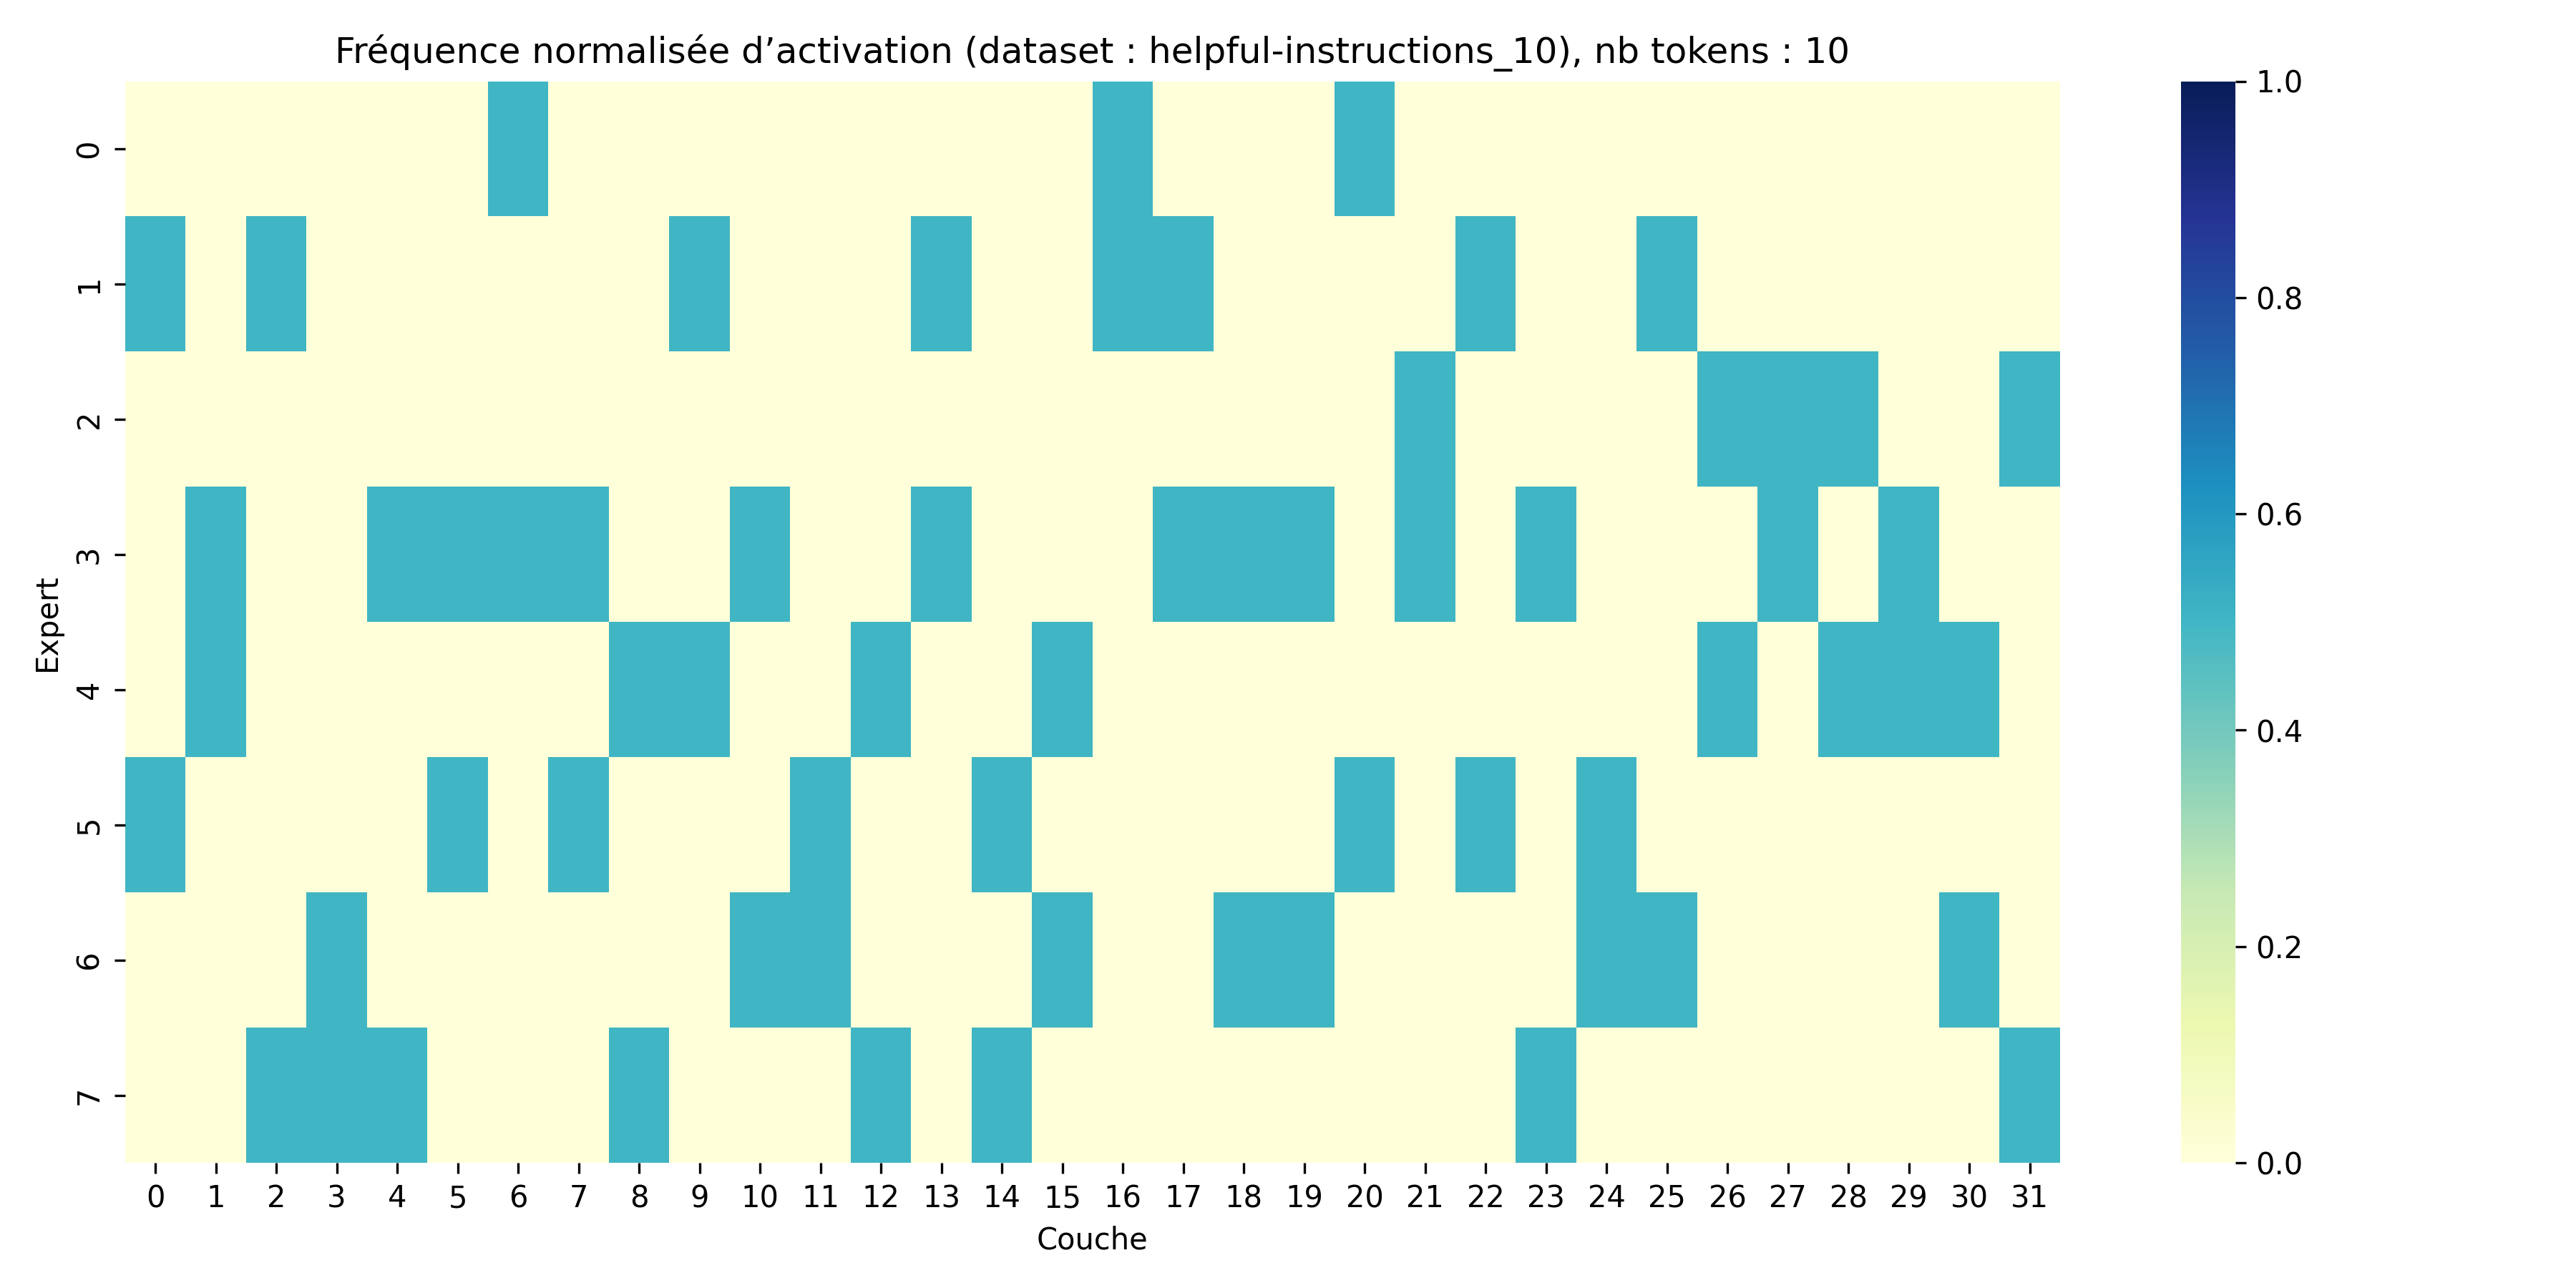
\includegraphics[width=.9\linewidth]{figures/Mixtral_8x7B/helpful_instr/10prompts/heatmap_tk1_experts_helpful-instructions_10.png}%
  }{%
    \begin{tcolorbox}[colback=yellow!5,colframe=yellow!50!black]
      Image manquante: heatmap token de démarrage
    \end{tcolorbox}}
  \caption{Utilisation des experts pour le token de démarrage.}
  \label{fig:heatmap_start}
\end{figure}

\begin{figure}[ht]
  \centering
  \IfFileExists{figures/Mixtral_8x7B/helpful_instr/10prompts/heatmap_tk28725_experts_helpful-instructions_10.png}{%
    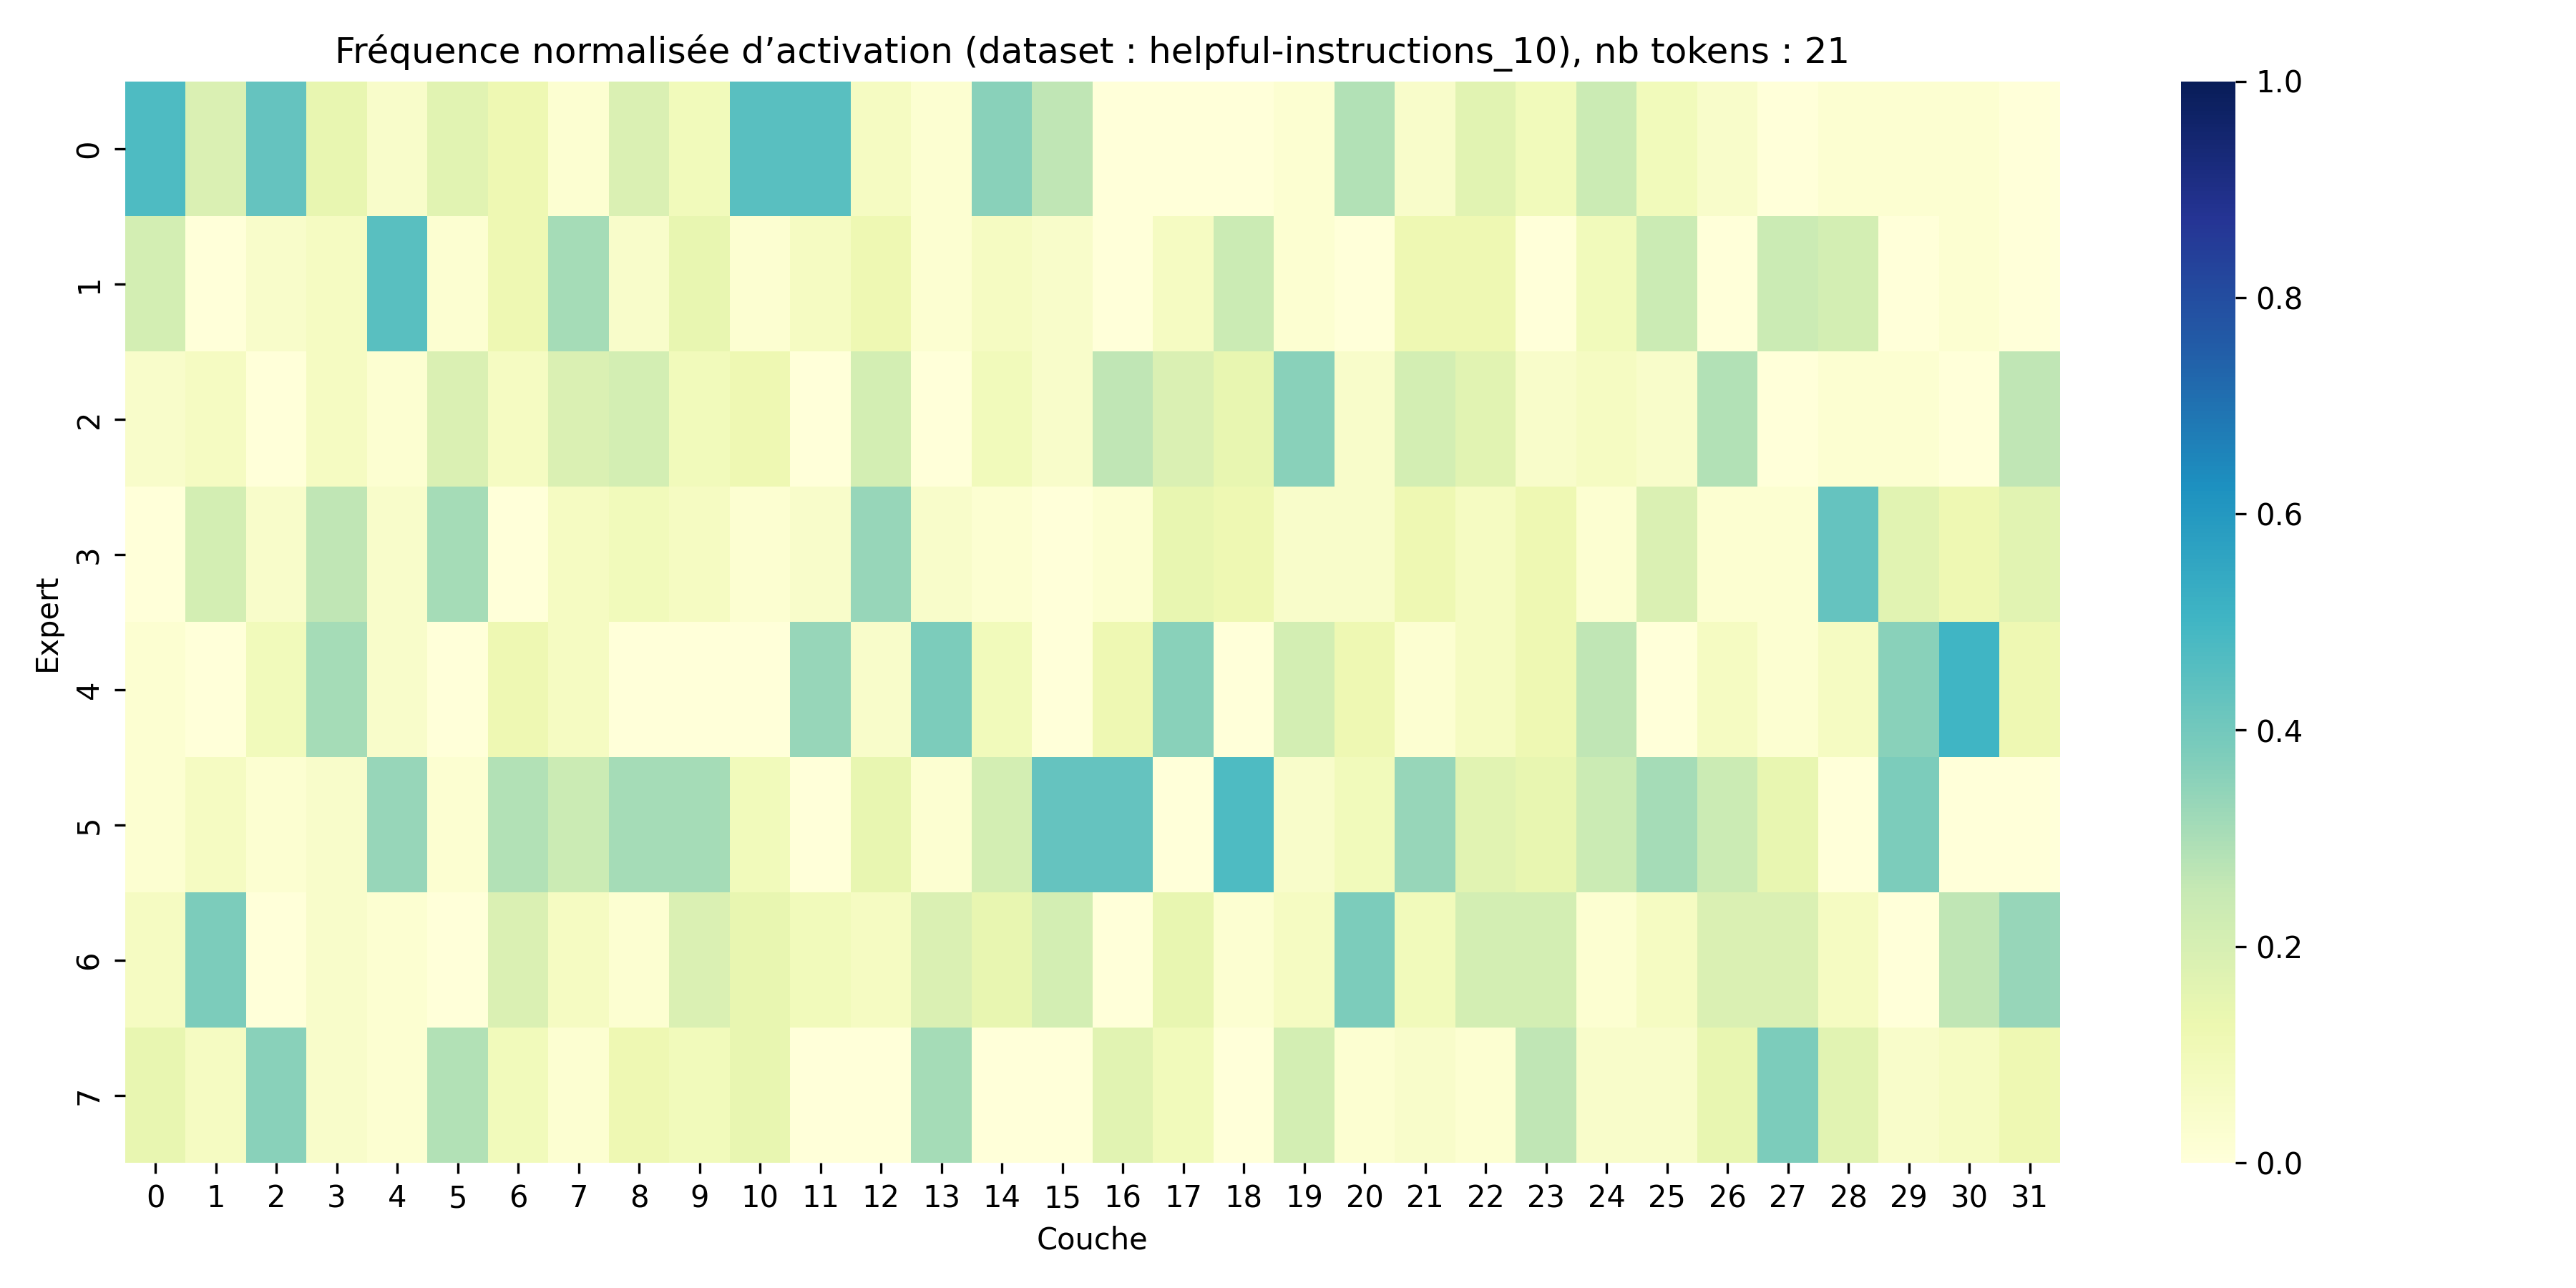
\includegraphics[width=.9\linewidth]{figures/Mixtral_8x7B/helpful_instr/10prompts/heatmap_tk28725_experts_helpful-instructions_10.png}%
  }{%
    \begin{tcolorbox}[colback=yellow!5,colframe=yellow!50!black]
      Image manquante: heatmap token virgule
    \end{tcolorbox}}
  \caption{Utilisation des experts pour le token virgule (,).}
  \label{fig:heatmap_comma}
\end{figure}

\subsection{Matrice de co-occurrence}
\begin{figure}[ht]
  \centering
  \IfFileExists{figures/cooccurrence_matrix.png}{%
    \includegraphics[width=.9\linewidth]{figures/cooccurrence_matrix.png}%
  }{%
    \begin{tcolorbox}[colback=yellow!5,colframe=yellow!50!black]
      Image manquante: \texttt{figures/cooccurrence_matrix.png}
    \end{tcolorbox}}
  \caption{Matrice de co-occurrence inter-couches (gauche : probabilité jointe ; droite : conditionnelle).}
  \label{fig:cooc}
\end{figure}

% =============================================================
\section{Résultats}

\subsection{Précision de la prédiction (exemples indicatifs)}
\begin{table}[ht]
  \centering
  \caption{Taux de \emph{hit} (\%) pour la prédiction spatiale (à actualiser)}
  \label{tab:hitrate}
  \begin{tabular}{lcc}
    \toprule
    \textbf{Approche} & \textbf{Top-1} & \textbf{Top-2} \\
    \midrule
    Gating inter-couches ($n{=}1$)      & 96.1 & 90.4 \\
    Réseau prédictif (V1 MLP)           & 97.3 & 92.7 \\
    Statistiques (couples majoritaires) & 85.8 & 78.2 \\
    \bottomrule
  \end{tabular}
\end{table}

\subsection{Impact sur le temps d'inférence (indicatif)}
En pré-chargeant les deux experts prédits une couche avant leur utilisation effective, on observe une baisse de latence typique de l’ordre de 14\,\% sur un batch de 128 tokens (GPU A100, FP16).

% =============================================================
\section{Discussion}

\paragraph{Difficultés.} Données déséquilibrées (longue traîne) ; sensibilité de certaines couches au \emph{noisy gating} ; définition de la cible (paire unique vs deux experts indépendants).
\paragraph{Limites.} Résultats \emph{in-domain} (helpful-instructions) — transférabilité à tester ; valeurs numériques ci-dessus à actualiser avec le protocole final.
\paragraph{Perspectives.} GRU/mini-Transformer ; loss plus proche du \emph{hit} (pénalisation de la paire erronée) ; déclenchement de préchargement par seuils de confiance ; études cross-dataset et cross-modèle.

% =============================================================
\section{Conclusion}
Nous montrons l’existence d’un \emph{signal exploitable} dans le contexte immédiat pour prédire les experts activés dans un LLM MoE. Les heuristiques statistiques donnent une base interprétable, tandis que le LSTM + réduction d’embeddings fournit la \emph{généralisation} nécessaire avec un coût maîtrisé (PCA). Ces résultats ouvrent des pistes concrètes de \emph{préchargement d’experts} et d’analyse du routage.

\newpage
\printbibliography

% =============================================================
% ANNEXE (optionnelle)
% =============================================================
\appendix
\section*{Annexe}
\begin{lstlisting}[caption={Estimation de la corrélation d'énergie (placeholder)}, label=lst:energy_estimation]
% CODE (à insérer)
\end{lstlisting}

\end{document}

